\chapter{Fundamentos:}

\section{El Qubit: Quantum Bit}
Un bit cuántico (\emph{qubit}) se describe por un \emph{estado} de dimensión 2. 
Un bit  clásico puede solo tomar valores 0 o 1. De igual forma un qubit puede estar en el estado $\ket{0}$ o $\ket{1}$, que corresponden a los estados de un bit clásico 0 y 1. La diferencia entre un bit y un qubit, es que el qubit puede estar en una \emph{superposición} de $\ket{0}$ y $\ket{1}$ al mismo tiempo.
Este fenómeno se lo puede observar tanto en el espín de un electrón como en la polarización de un fotón. El estado de un qubit se puede describir de la siguiente manera:
\begin{equation}
  \ket{\psi} = \alpha\ket{0} + \beta\ket{1},
\end{equation}
donde $\alpha$ y $\beta$ son números complejos. Aquí $\alpha$ y $\beta$ son las \emph{amplitudes de probabilidad}, y $\ket{0}$, $\ket{1}$ se denominan estados de la \emph{base estándar computacional}.

Las amplitudes de un qubit no se pueden determinar directamente, es necesario medirlo. Si lo medimos, podemos obtener $\ket{0}$ con probabilidad $|\alpha|^2$, o $\ket{1}$ con probabilidad $|\beta|^2$. 
La suma de los valores absolutos al cuadrado de las amplitudes siempre suman 1 por el hecho de tratarse de probabilidades. Esto está garantizado por la condición de normalización de los estados físicos, anteriormente mencionada ($|\alpha|^2 + |\beta|^2 = 1$).

Por ejemplo midiendo al qubit en el estado
\begin{equation}
  \dfrac{1}{\sqrt2}\ket{0}+\dfrac{1}{\sqrt2}\ket{1}
\end{equation}
se obtiene $\ket{0}$ la mitad de las veces y $\ket{1}$ la otra mitad ($|1/\sqrt2|^2 = 0.5$). Este estado se lo denota $\ket{+}$.

\subsection{La Esfera de Bloch}
La esfera de Bloch es la representación geométrica del estado de un qubit. Es un sistema de coordenadas esféricas en el cual un estado cuántico se lo puede describir como
\begin{equation}
  \ket{\psi} = e^{i\delta} \left(\cos\dfrac{\theta}{2}\ket{0} + e^{i\phi}\sin\dfrac{\theta}{2}\ket{1}\right),
\end{equation}
donde $\delta, \theta$ y $\phi$ son números reales. 
El factor $e^{i\delta}$ es una fase global del estado. 
Este factor no influye en las probabilidades de medida, ya que $\left|e^{i\delta}\right| = 1$, por lo que es usual omitirlo, permitiéndonos escribir
\begin{equation}
  \ket{\psi} = \cos\dfrac{\theta}{2}\ket{0} + e^{i\phi}\sin\dfrac{\theta}{2}\ket{1}.
\end{equation}
Los números $\theta$ y $\phi$ definen un punto en la esfera tridimensional (Figure~\ref{fig:bloch}). 
La esfera de Bloch es muy útil para visualizar operaciones de un qubit. Sin embargo, existen limitaciones para generalizar la esfera de Bloch a muchos qubits.
\begin{figure}[ht]
  \centering
  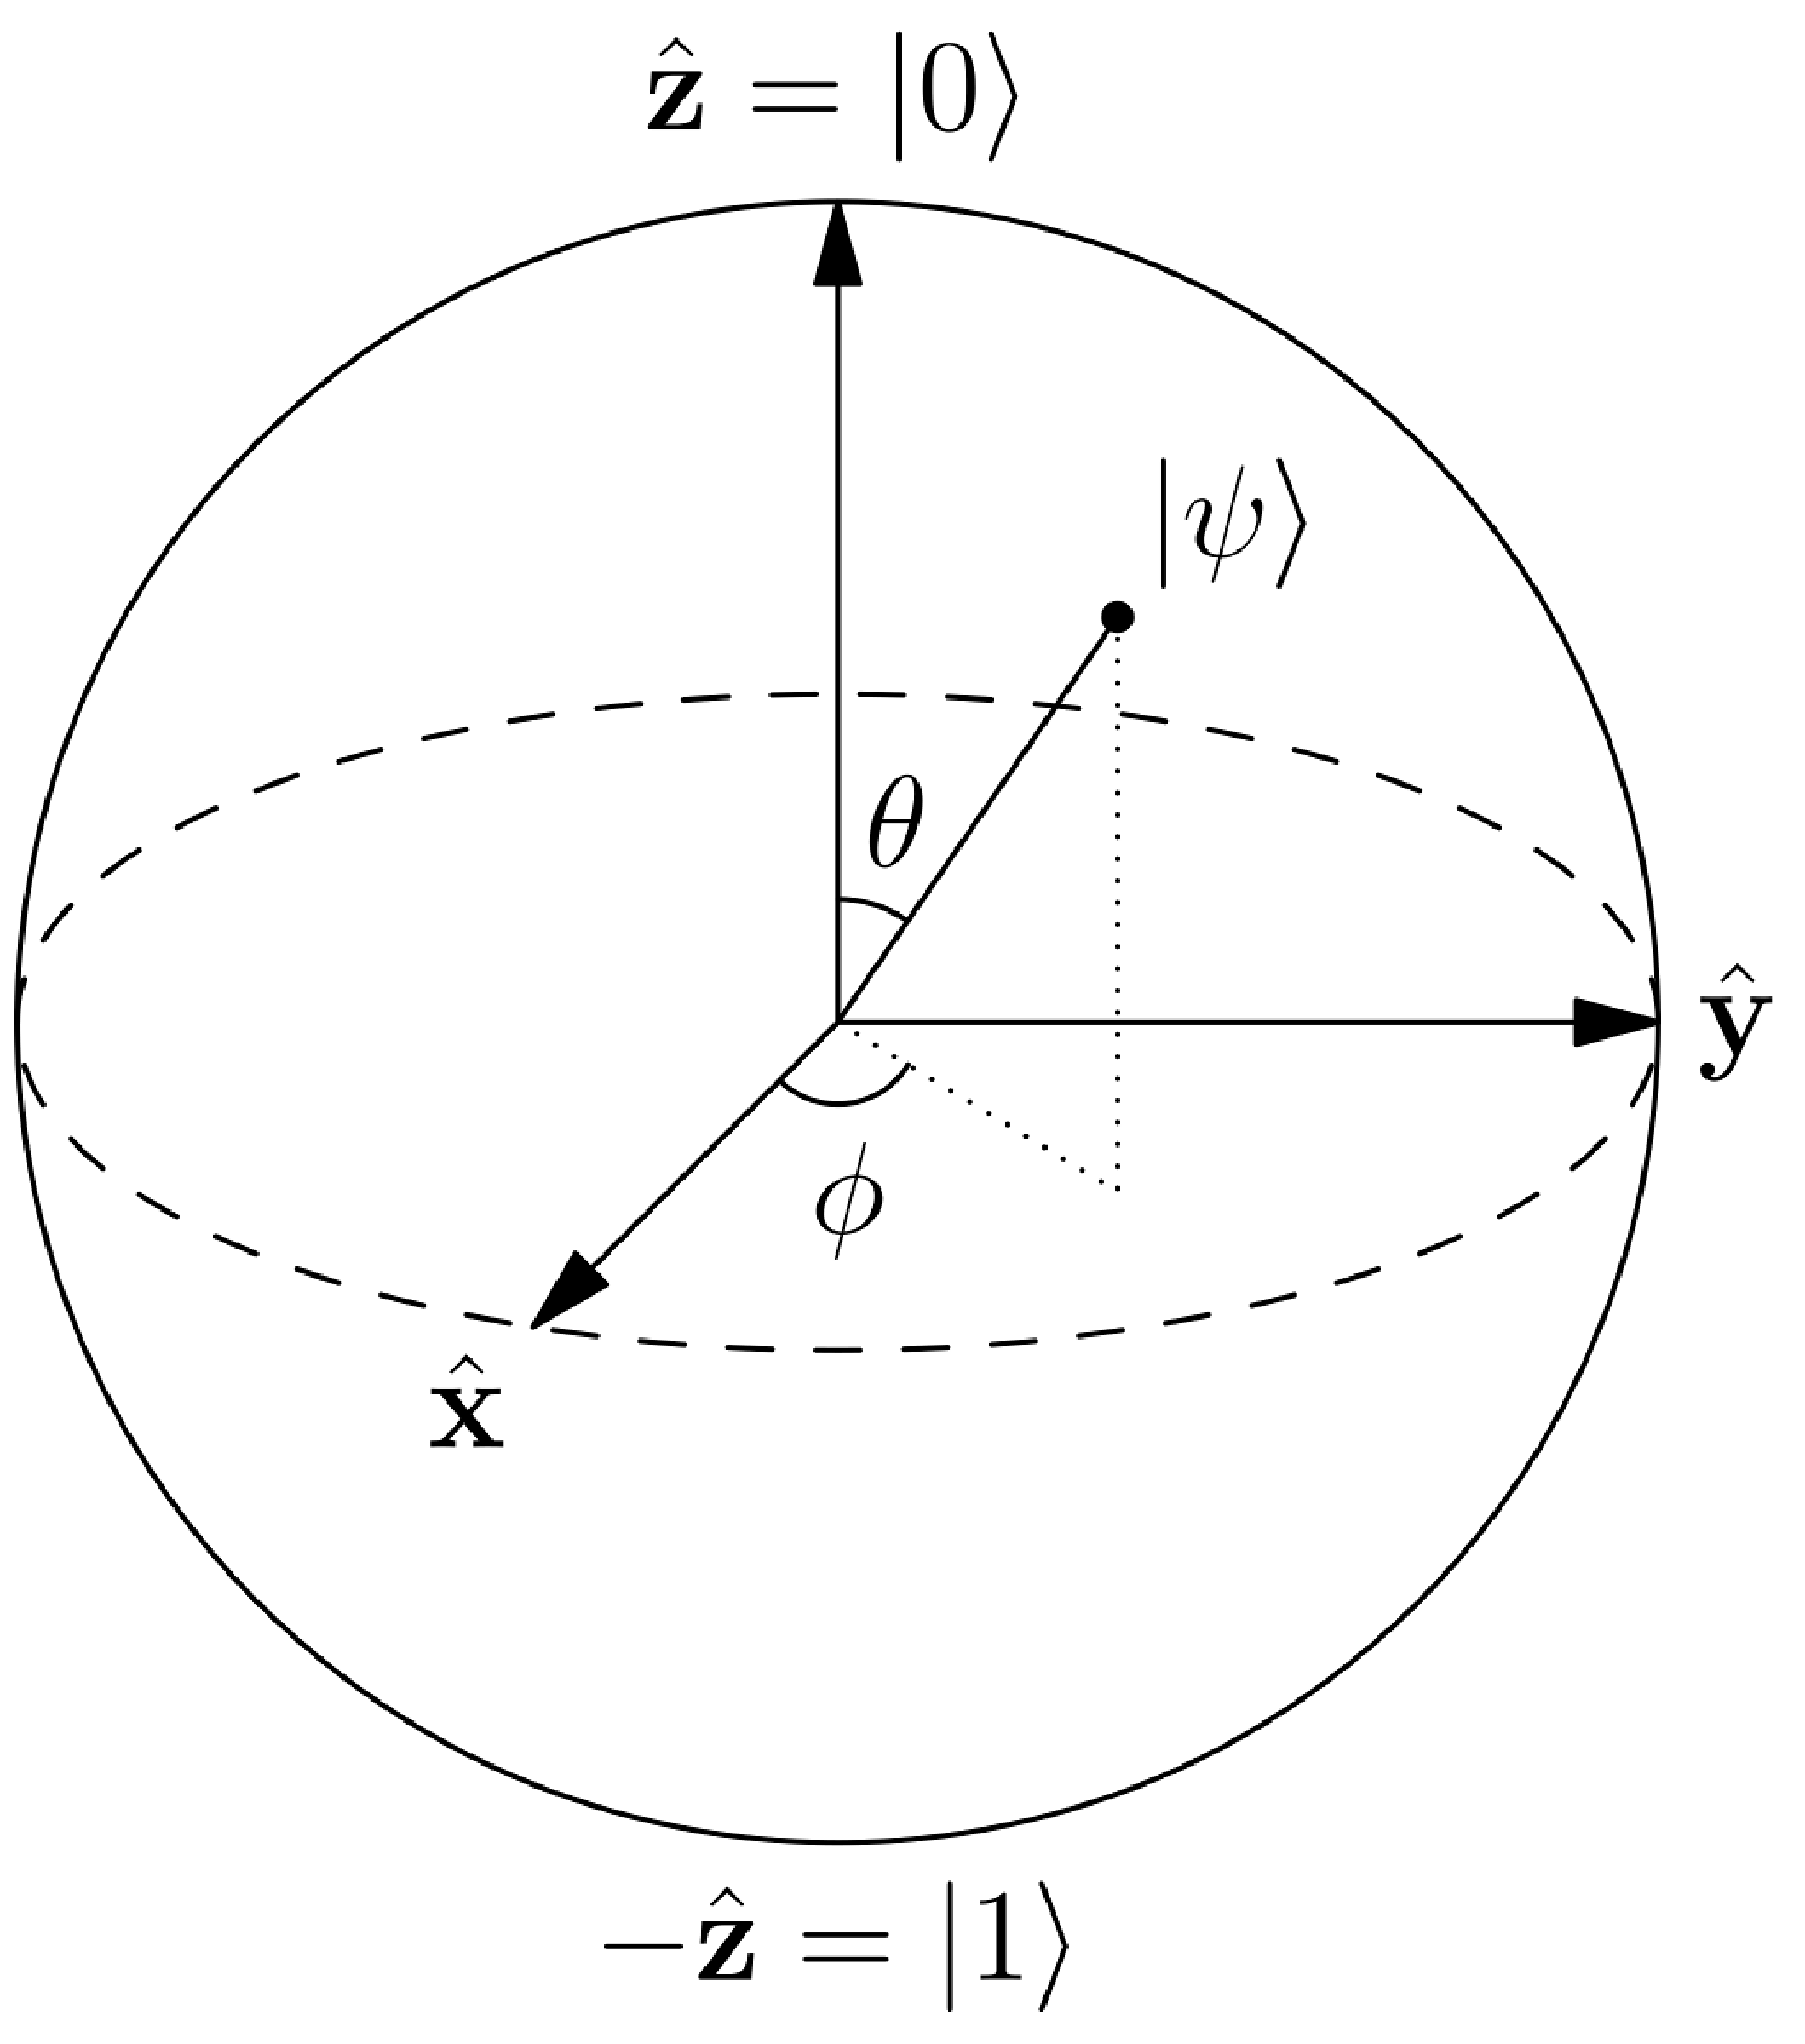
\includegraphics[scale=0.175]{Figures/bloch-sphere.eps}
  \vspace{2mm}
  \caption{Representación de un qubit en la esfera de Bloch.}
  \label{fig:bloch}
\end{figure}

\subsection{Compuertas de un qubit: Single-Qubit Gates}
Las compuertas de un qubit se pueden ver como rotaciones en la esfera de Bloch. Estas compuertas son \emph{unitarias}, es decir $U^\dagger U = UU^\dagger = I$, donde $U^\dagger$ es
la transpuesta conjugada de $U$ y $I$ la identidad. Por lo que cualquier unitaria de $2^n \times 2^n$ es una compuerta válida que actúa en $n$ qubits. Comúnmente $\ket{\psi'} = U\ket{\psi}$ se representan a través un circuito:
\begin{center}
\begin{quantikz}
\lstick{$\ket{\psi}$} & \gate{U} & \qw & \rstick{$\ket{\psi'}$}\qw
\end{quantikz}
\end{center}
% \[
%   \Large
%   \Qcircuit @C=1em @R=0em {
%     & \lstick{\ket{\psi}} & \gate{U} & \qw & \ket{\psi'}
%   }
% \]
A continuación se describen y visualizan algunas compuertas de un qubit usuales.

\subsection{Compuertas de Pauli}\label{pauli_gates}
 Las compuertas de un qubit más simples son las matrices de \emph{Pauli:} $I$, $X$, $Y$ y $Z$. Donde $I$ es la identidad y las compuertas $X$, $Y$ y $Z$ rotan $\pi$ radianes alrededor de los ejes X, Y o Z, respectivamente. 
 
\begin{figure}[ht]
  \centering
  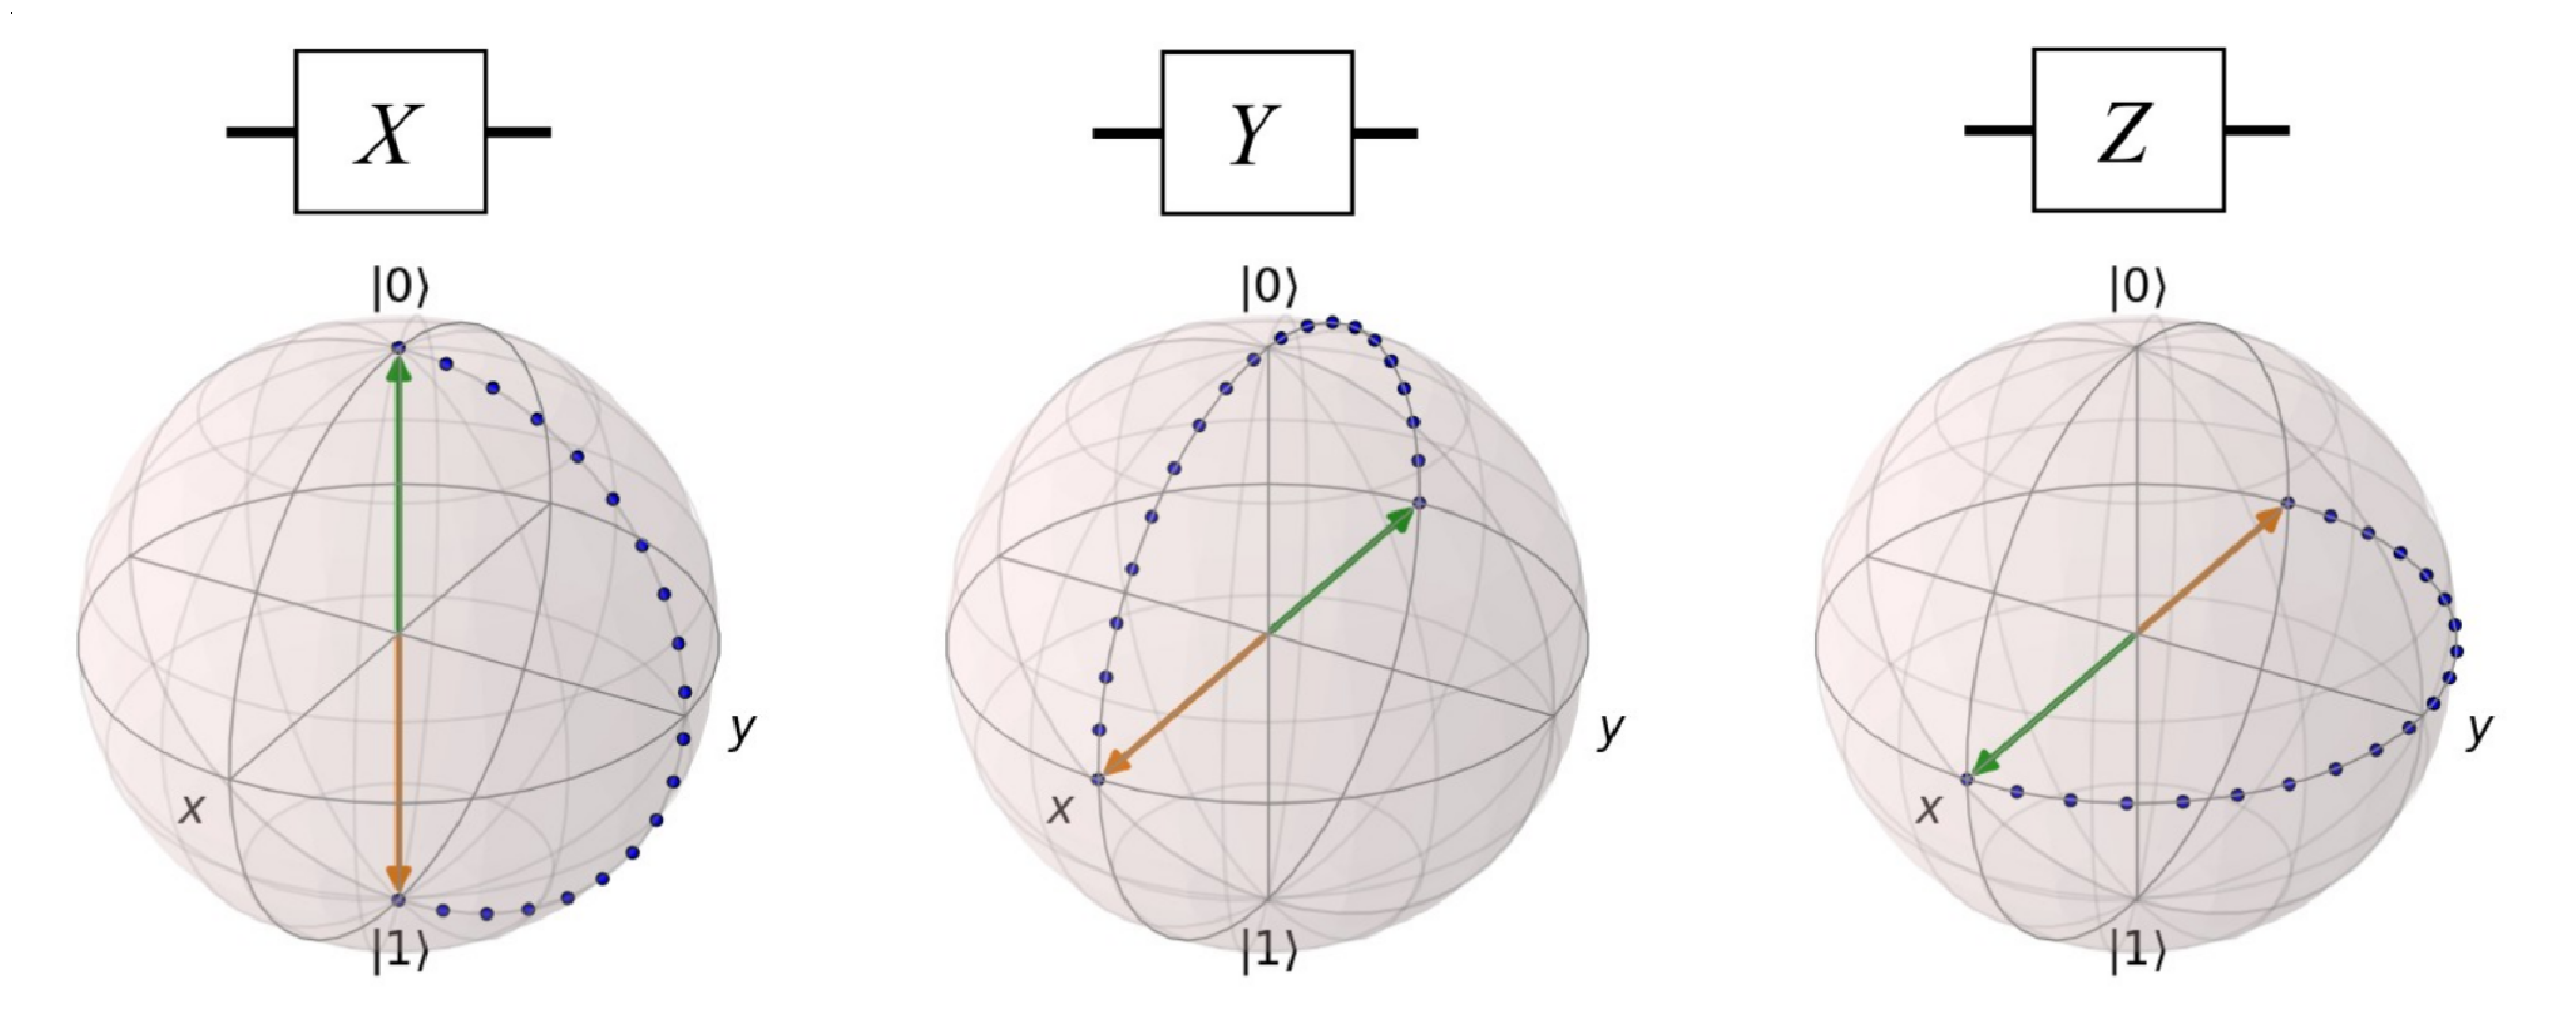
\includegraphics[scale=0.175]{pauli-gates.eps}
  \vspace{2mm}
  \caption{Compuertas $X$, $Y$ y $Z$ visualizadas en la esfera de Bloch. El vector inicial está en verde y el naranja es el de la posición final.}
\end{figure}

\subsection{Compuerta Hadamard}
La compuerta \emph{Hadamard} ($H$) (Figura \ref{fig:hadamard_bloch}) mapea los estados de la base estándar $\ket{0}$ y $\ket{1}$ a estados de superposición con pesos iguales:
\begin{align}
  H\ket{0} &= \dfrac{1}{\sqrt2}(\ket{0} + \ket{1}) = \ket{+} \\
  H\ket{1} &= \dfrac{1}{\sqrt2}(\ket{0} - \ket{1}) = \ket{-}.
\end{align}
Es la combinación de dos rotaciones  de $\pi$ alrededor del eje Z seguidas de una $\pi/2$ alrededor del eje. También se la puede ver como una rotación de $\pi$ alrededor del eje $n=(1,0,1)/\sqrt{2}$.

\begin{figure}[ht]
  \centering
  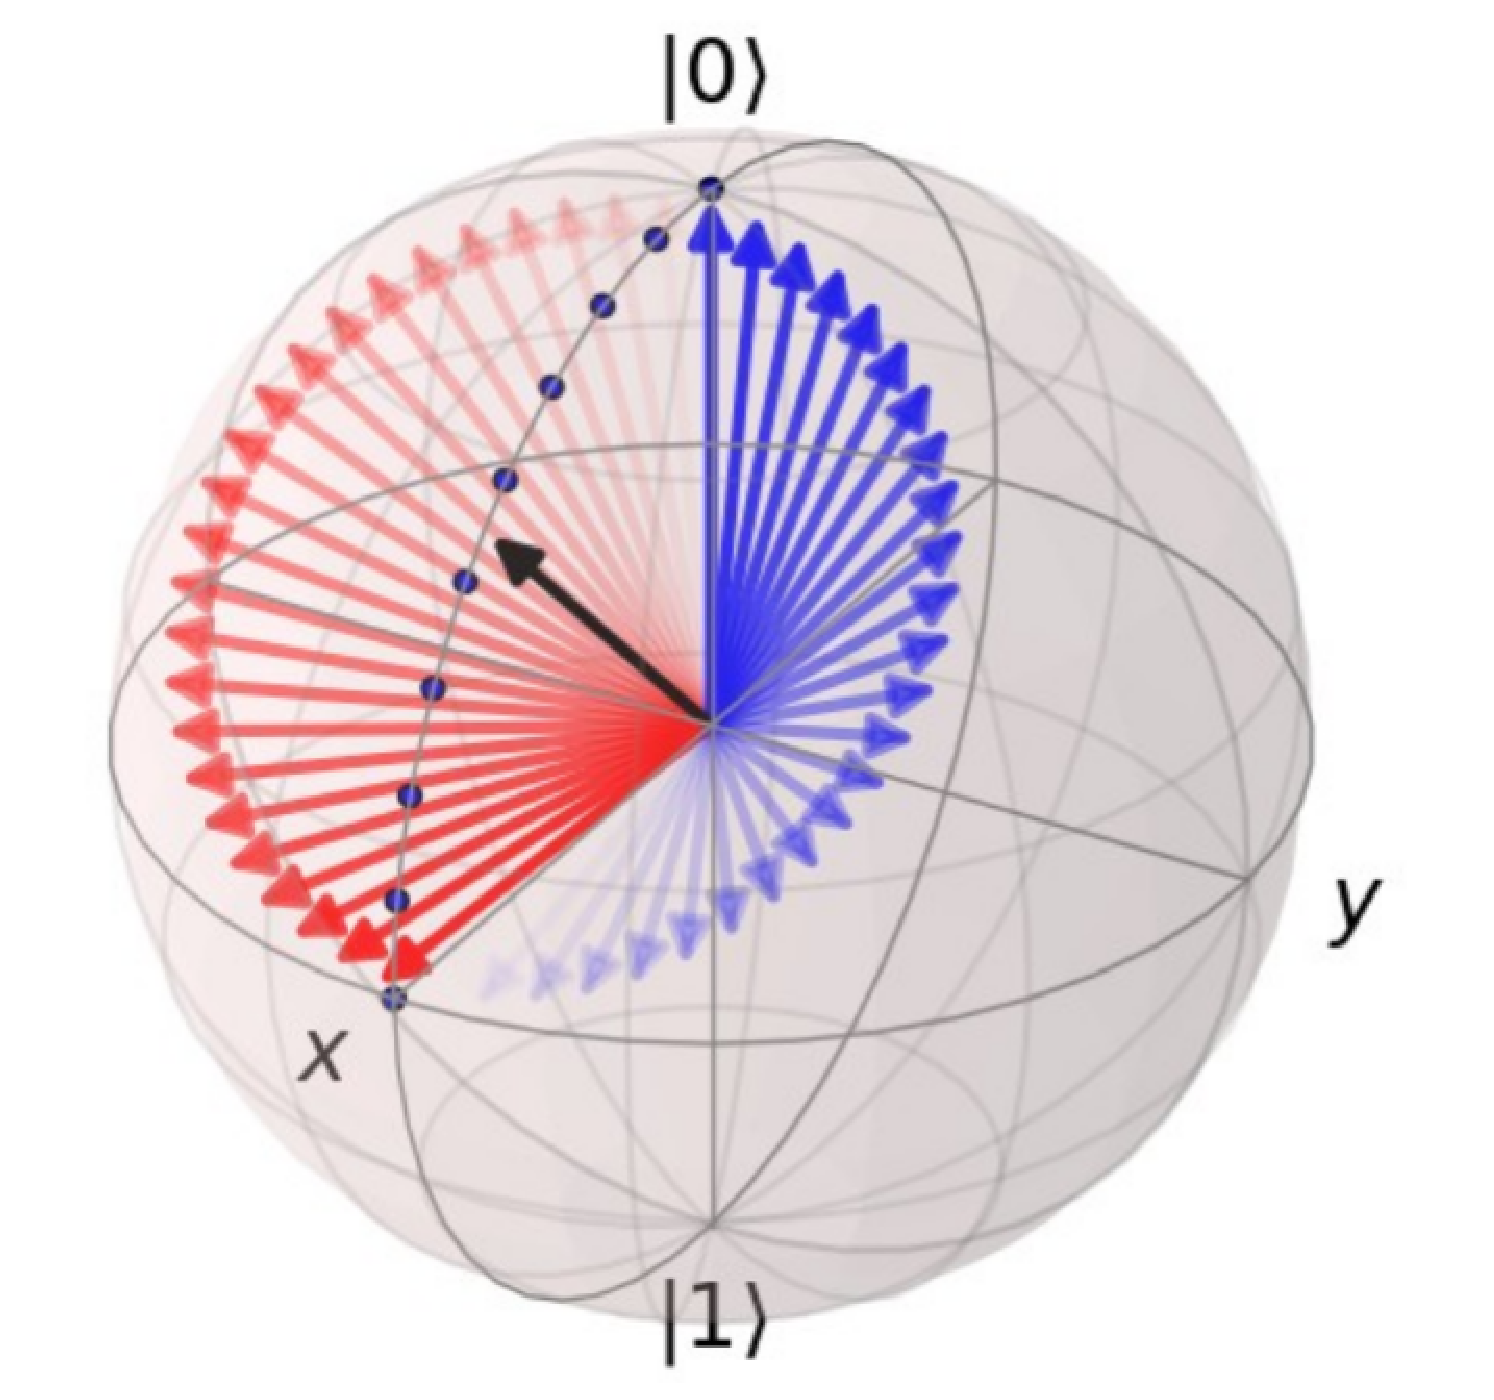
\includegraphics[scale=0.17]{hadamard-gate.eps}
  \vspace{1mm}
  \caption{Visualización de la compuerta Hadamard en la esfera de Bloch.}
  \label{fig:hadamard_bloch}
\end{figure}

\subsection{Compuerta Fase}
Compuertas de que rotan alrededor del eje Z se llaman \emph{Compuertas Fase}. Rotan la fase del estado $\ket{1}$
un ángulo $\theta$ dejando igual al estado $\ket{0}$:
\begin{equation}
  \begin{aligned}
    R_z(\theta) \ket{0} &= \ket{0} \\
    R_z(\theta) \ket{1} &= e^{i\theta}\ket{1}.
  \end{aligned}
\end{equation}
La probabilidad de medir $\ket{0}$ o $\ket{1}$ no cambia al aplicar la compuerta fase, como su nombre lo indica solo cambia la fase del estado cuántico. Una compuerta fase común es la compuerta $S$, donde $\theta = \pi/2$ (Figure \ref{fig:s_bloch}). La compuerta Pauli Z 
se puede pensar como una compuerta fase con $\theta = \pi$ (dado que $e^{i\pi} = -1$). Por lo que se puede pensar a la compuerta $S$ como la mitad de la compuerta $Z$.
Otra compuerta fase conocida es la compuerta $T$,
donde $\theta = \pi/4$ (la mitad de una compuerta $S$).

\begin{figure}[ht]
  \centering
  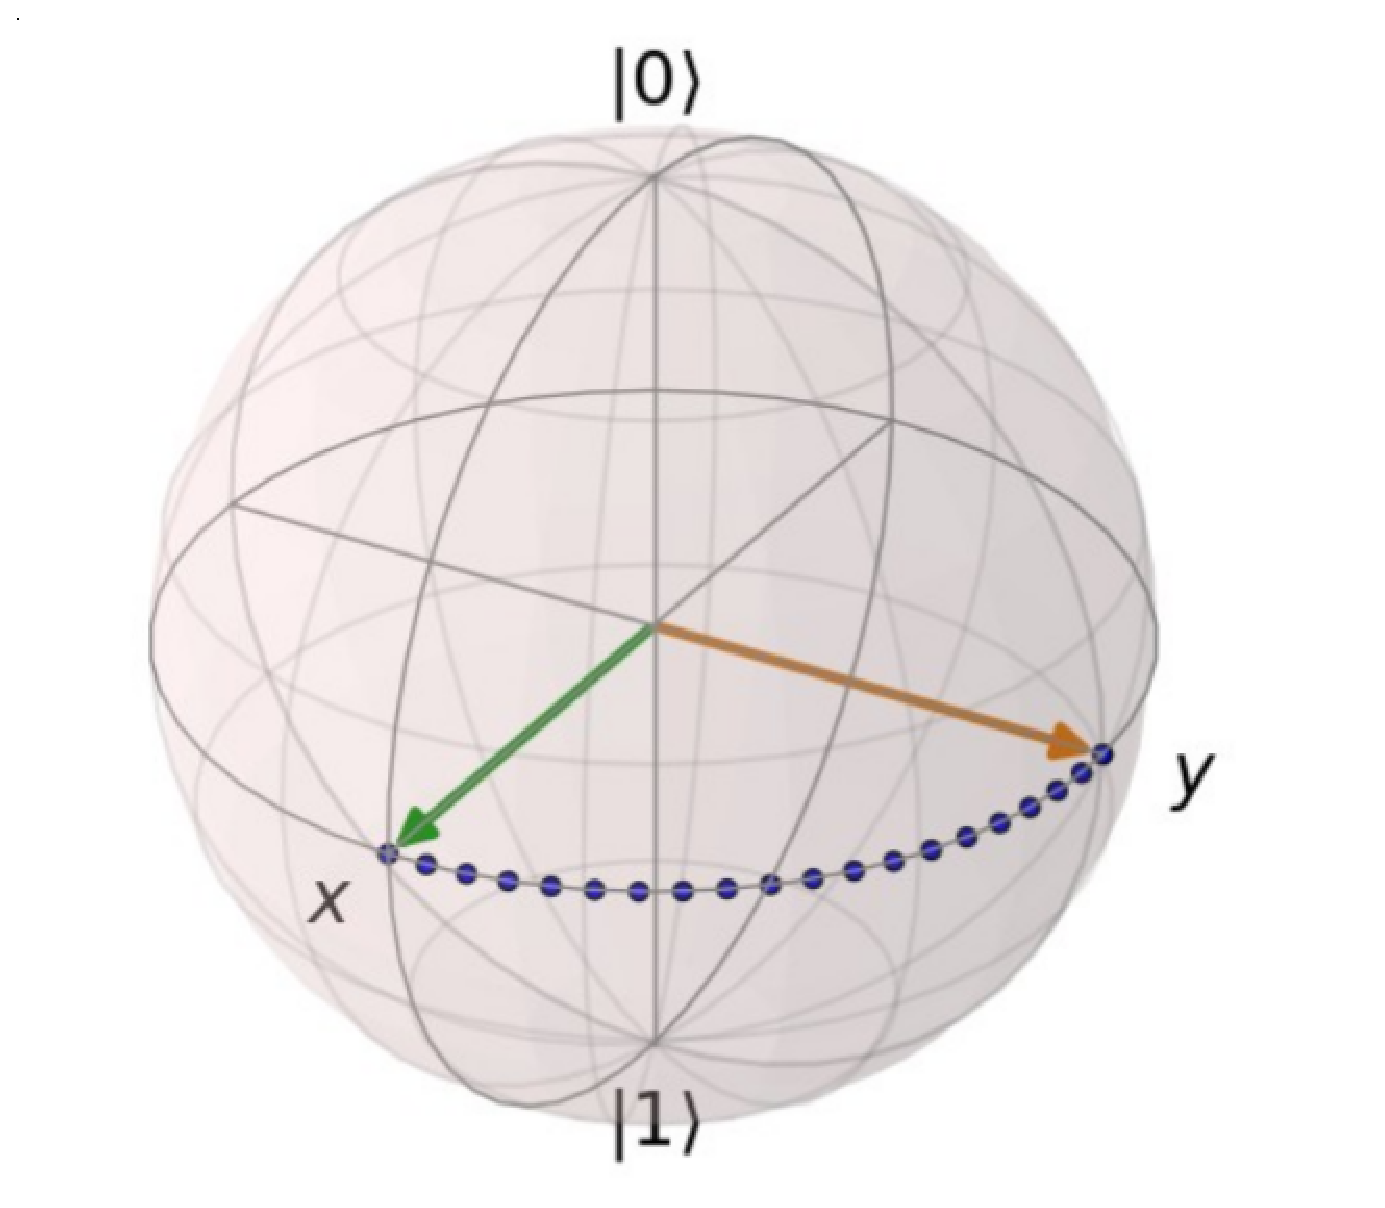
\includegraphics[scale=0.21]{s-gate.eps}
  \vspace{1mm}
  \caption{Visualización de la compuerta $S$ en la esfera de Bloch.}
  \label{fig:s_bloch}
\end{figure}


\subsection{Medida de un qubit}
En la sección (\ref{medidas}) se introdujo la idea de medida en mecánica cuántica, aquí vemos su aplicación más simple que es el caso de medir un qubit.
Al medir un qubit $\ket{\psi}$ en la base computacional, la superposición cuántica colapsa a un estado de la base. Se dice que estado $\ket{\psi}$ ``colapsó", quedando en el estado$\ket{0}$ o $\ket{1}$. Se puede calcular la probabilidad de que se obtenga cierto resultado de la medida a través de las amplitudes de probabilidad:
\begin{align}
  P(\ket{0}) &= \left|\alpha\right|^2 \\
  P(\ket{1}) &= \left|\beta\right|^2.
\end{align}

Esto se puede observar en el circuito simple de un qubit:

\begin{figure}[ht]
\begin{center}
\begin{quantikz}
\lstick{$\ket{0}$} & \gate{H} & \gate{Z} & \meter{} & \qwbundle[alternate=2]{}
\end{quantikz}
% \begin{quantikz}
% \lstick{$\ket{0}$} & \gate{H} & \gate{Z} & \meter\qwbundle[alternate=2]{} & \qwbundle[alternate=2]{} 
% \end{quantikz}
\end{center}
\caption{El resultado de la medida de un qubit es un bit clásico, que se diferencia de un qubit representándolo con un cable doble. Este circuito se puede visualizar en la esfera de Bloch en la Figura~\ref{fig:gate_rotations}.}
\end{figure}
\noindent

En primer lugar se calcula $H\ket{0} = \ket{+}$, seguido de $Z\ket{+} = (\ket{0} - \ket{1})/\sqrt 2$, (o $\ket{-}$). Finalmente se mide, obteniendo algún estado de la base computacional $\ket{j}$.
Lo único que se puede afirmar es que se obtendrá el estado $\ket{j}$ con probabilidad $|a_j|^2$:
\begin{align}
  P(\ket{0}) = \left|\dfrac{1}{\sqrt2}\right|^2 &= \dfrac{1}{2} \\
  P(\ket{1}) = \left|\dfrac{-1}{\sqrt2}\right|^2 &= \dfrac{1}{2}.
\end{align}
Teniendo igual probabilidad de medir $\ket{0}$ o $\ket{1}$.

\begin{figure}[ht]
  \centering
  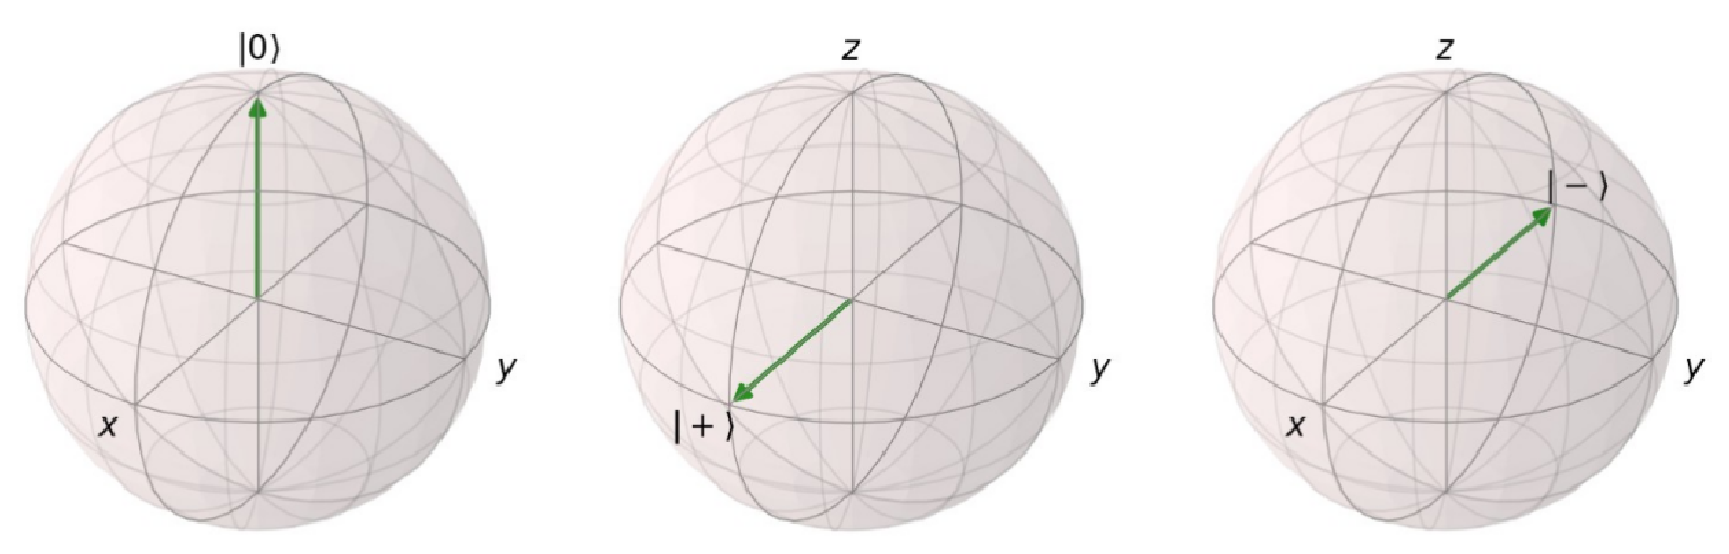
\includegraphics[scale=0.375]{simple-circuit.eps}
  \vspace{2mm}
  \caption{Estados del qubit a través del circuito: $\ket{0}$ $\rightarrow$ $H\ket{0}$ $\rightarrow$ $ZH\ket{0}$.}
  \label{fig:gate_rotations}
\end{figure}

\subsection{Notación Vectorial} \label{sec:matrix_notation}
Anteriormente vimos que un estado de un qubit se puede escribir como
\begin{equation}
  \ket{\psi} = \alpha\ket{0} + \beta\ket{1}.
\end{equation}
Los kets $\ket{0}$ y $\ket{1}$ forman la base estándar de un qubit y se representan como:
\setlength\multicolsep{0pt}
\begin{equation}
  \ket{0} = \qstatezero{}; \quad \ket{1} = \qstateone{}.
\end{equation}
\noindent
Como ya se mencionó un estado cuántico debe estar normalizado por lo que el estado de un qubit es un vector normalizado de un espacio vectorial complejo de dimensión 2. Un estado de $n$ qubits tiene un \emph{espacio de Hilbert} de dimensión $2^n$.  Un estado cuántico se puede escribir como combinación lineal de estados de la base:
\begin{equation}
  \ket{\psi} = \alpha\qstatezero{} + \beta\qstateone{} = \begin{pmatrix}\alpha \\ \beta\end{pmatrix}.
\end{equation}
Por lo que las compuertas de un qubit se pueden representar por matrices unitarias de $2 \times 2$:
\vspace*{-4mm}
\setlength\multicolsep{0pt}
\begin{multicols}{3}
  \[
    I = \igate{};
  \]
  \vfill
  \[
    X = \xgate{};
  \]
  \vfill
  \[
    Y = \ygate{};
  \]
\end{multicols}
\begin{multicols}{3}
  \[
    Z = \zgate{};
  \]
  \vfill
  \[
    S = \sgate{};
  \]
  \vfill
  \[
    H = \hgate{}.
  \]
\end{multicols}
\bigskip
\noindent
Luego, aplicar la compuerta $X$ al estado $\ket{0}$, $X \ket{0}$ se puede calcular simplemente como una multiplicación de una matriz por un vector:
\begin{equation}
  X\ket{0} = \xgate{} \qstatezero{} = \qstateone{}.
\end{equation}
Por lo que vemos que $X\ket{0} = \ket{1}$. De forma general:
\begin{equation}
  X\begin{pmatrix}\alpha \\ \beta\end{pmatrix} = \begin{pmatrix}\beta \\ \alpha\end{pmatrix}.
\end{equation}

Las compuertas cuánticas se pueden combinar multiplicando sus respectivas matrices. Por ejemplo,
podemos verificar que la compuerta Hadamard es su propia inversa:
\begin{equation}
  H^2 = \hgate{} \hgate{} = \igate{} = I.
\end{equation}
Es a su vez una \emph{matriz Hermítica}, ya que es igual a su propia transpuesta conjugada: $H = H^\dagger$.

\section{Multi-Qubits}
Para representar más de un qubit se utiliza el \emph{producto tensorial}. Dadas $A$ una matriz de  $m \times n$ y $B$ una matriz de $p \times q$, luego
\begin{equation}
  A \otimes B = \begin{pmatrix}
      a_{11} & \dots & a_{1n} \\
      \vdots & \ddots & \vdots \\
      a_{m1} & \dots & a_{mn} \\
    \end{pmatrix} \otimes B =
    \begin{pmatrix}
      a_{11}B & \dots & a_{1n}B \\
      \vdots & \ddots & \vdots \\
      a_{m1}B & \dots & a_{mn}B \\
    \end{pmatrix},
\end{equation}
resultando en un matriz de $mp \times nq$.
Se puede representar el estado de dos qubits $\ket{00}$ como
\begin{equation}
  \ket{00} = \ket{0} \otimes \ket{0} = \qstatezero{} \otimes \qstatezero{} =
  \begin{pmatrix}
    1\qstatezero{} \\[13pt]
    0\qstatezero{}
  \end{pmatrix}
  =
  \begin{pmatrix}
    1 \\
    0 \\
    0 \\
    0
  \end{pmatrix}.
\end{equation}
Las notaciones: $\ket{00} = \ket{0}\!\ket{0} = \ket{0} \otimes \ket{0}$, son equivalentes.
El estado de dos qubits se puede escribir como:
\begin{equation}
  \ket{ab} = \ket{a} \otimes \ket{b} = \alpha_{00}\ket{00} + \alpha_{01}\ket{01} + \alpha_{10}\ket{10} + \alpha_{11}\ket{11}.
\end{equation}
Un estado en general se puede escribir como combinación lineal $\sum_{j} \alpha_j\ket{\psi_j}$ de estados $\ket{\psi_j}$ con sus amplitudes correspondientes $\alpha_j$.

Notar que a diferencia de los bits clásicos, el espacio de un estado crece de forma exponencial con el número de qubits, con $n$ qubits se pueden representar $2^n$ estados. Estados de muchos qubits, como cualquier estado cuántico tienen que estar normalizado. Para un estado de $n$ qubits:
\begin{equation}
  \sum_{j = 0}^{2^n-1} |\alpha_j|^2 = 1.
\end{equation}

\subsection{Evolución de un estado de dos qubits}
En la sección (\ref{evol}) se introdujo el concepto de evolución de un sistema cuántico cerrado, en esta sección veremos un ejemplo en el caso de dos qubits en el que la unitaria es simplemente aplicarle la compuerta $H$ al segundo, $H_1\ket{0_0 0_1}$.Esto se puede obtener de forma simple:
\begin{equation}
  H_1\ket{0_0 0_1} = (I_0 \otimes H_1)\ket{0_0 0_1}.
\end{equation}
Si se quiere calcular la matriz explícitamente:
\begin{align}
  I_0 \otimes H_1 &=
  \igate{} \otimes \hgate{} \\
  &=
  \dfrac{1}{\sqrt2}
  \left[
    \igate{}
    \otimes
    \begin{pmatrix}
      1 & \phantom{-}1 \\
      1 & -1
    \end{pmatrix}
  \right] \\
&= \dfrac{1}{\sqrt2}
  \begin{pmatrix}
    1 & \phantom{-}1 & 0 & \phantom{-}0 \\
    1 & -1 & 0 & \phantom{-}0 \\
    0 & \phantom{-}0 & 1 & \phantom{-}1 \\
    0 & \phantom{-}0 & 1 & -1 \\
  \end{pmatrix}.
\end{align}
Por lo que vemos que $I_0 \otimes H_1 \ket{00}$:
\begin{equation}
  \dfrac{1}{\sqrt2}
  \begin{pmatrix}
    1 & \phantom{-}1 & 0 & \phantom{-}0 \\
    1 & -1 & 0 & \phantom{-}0 \\
    0 & \phantom{-}0 & 1 & \phantom{-}1 \\
    0 & \phantom{-}0 & 1 & -1 \\
  \end{pmatrix}
  \begin{pmatrix}
    1 \\
    0 \\
    0 \\
    0
  \end{pmatrix}
  =
  \dfrac{1}{\sqrt2}
  \begin{pmatrix}
    1 \\
    1 \\
    0 \\
    0
  \end{pmatrix},
\end{equation}
 da como resultado el estado $(\ket{00} + \ket{01})/\sqrt2=\ket{0+}$, como era de esperarse.

\subsection{Medidas parciales de dos qubits}
Ya se introdujo el concepto de medidas en la sección (\ref{medidas}), en este caso vemos un ejemplo simple de dos qubits en el que se mide el qubit $\ket{q_0}$ como se observa en el circuito:
\begin{center}
\begin{quantikz}
\lstick{$\ket{q_0} = \ket{0}$} & \gate{H} & \meter{} \\
\lstick{$\ket{q_1} = \ket{0}$} & \gate{H} & \qw \\
\end{quantikz}
\end{center}

% \[
%   \Large
%   \Qcircuit @C=1em @R=0.5em {
%     \push{\rule{0em}{1.5em}} & & & & & \lstick{\ket{q_0} = \ket{0}} & \gate{H} & \meter & \cw \\
%     \push{\rule{0em}{1.5em}} & & & & & \lstick{\ket{q_1} = \ket{0}} & \gate{H} & \qw & \qw \\
%   }
% \]
\noindent
Inicialmente los dos qubits están en el estado $\ket{00}$ y se aplica la compuerta Hadamard a cada uno:
\begin{equation}
  (H \otimes H)\ket{00} = \dfrac{1}{2}(\ket{00} + \ket{01} + \ket{10} + \ket{11}).
\end{equation}
si se mide el $\ket{q_0}$ se tiene mitad de probabilidad de obtener $\ket{0}$ o $\ket{1}$. Al medir, el estado $\ket{q_0}$ colapsa a alguno de los siguientes estados:
\begin{equation}
  \ket{\psi} =
  \begin{cases}
    \begin{aligned}
      \dfrac{1}{\sqrt2}(\ket{\uline{0}0} + \ket{\uline{0}1}) & \text{ if } M(q_0) = \ket{0} \\
      \dfrac{1}{\sqrt2}(\ket{\uline{1}0} + \ket{\uline{1}1}) & \text{ if } M(q_0) = \ket{1}
    \end{aligned}
  \end{cases}
\end{equation}
Luego de la medida se tienen dos estados posibles para $\ket{q_0}$: $\ket{0}$ o $\ket{1}$. El qubit $\ket{q_1}$ 
quedará en una superposición porque no se lo midió. Notar que los primeros qubits (subrayados) en ambos estados son iguales. Lo cual tiene sentido porque se midió este qubit por lo que se tiene certeza sobre este estado.

\section{Compuertas de dos qubits usuales}
\subsection{Compuerta CNOT}
La compuerta cuántica control-\textsc{not} (\textsc{cnot}, a veces llamada control-$X$) 
es similar a la compuerta clásica \textsc{xor}, 
pero es reversible. Esta compuerta tiene dos qubits de entrada el qubit de \emph{control} y el qubit \emph{target}. Si el qubit de control está en 0, luego se deja igual al qubit target. Pero si el qubit de control está en 1, el qubit target se invierte. El circuito que representa al \textsc{cnot} se puede observar en la  Figura~\ref{fig:cnot_circuit}. El qubit $\ket{q_0}$ representa al qubit de control y $\ket{q_1}$ representa al qubit target. Es esencialmente una compuerta $X$ con un qubit de control. \textsc{cnot} es hermítica.

\begin{figure}[ht]
  \centering
  \begin{minipage}{.45\textwidth}
   \begin{center}
   \begin{quantikz}
   \lstick{$\ket{q_0}$} & \ctrl{1} & \ctrl{1} & \qw \\
   \lstick{$\ket{q_1}$} & \targ{} & \gate{X} & \qw \\
\end{quantikz}
\end{center}
    \caption{Dos formas diferentes de representar a \textsc{cnot} en un circuito.}
    \label{fig:cnot_circuit}
  \end{minipage}%
  \hspace*{.05\textwidth}
  \begin{minipage}{.45\textwidth}
    \[
      U_{\textsc{cnot}} = \cnotgate{}
    \]
  \caption{Representación matricial de \textsc{cnot}.}
  \end{minipage}
\end{figure}
\noindent
Veamos un ejemplo en el cual se utiliza la compuerta \textsc{cnot}. 
Consideramos el siguiente circuito:

\begin{center}
   \begin{quantikz}
   \lstick{$\ket{q_0}= \ket{0}$} & \gate{X} & \ctrl{1} & \ctrl{1} & \qw \\
   \lstick{$\ket{q_1}= \ket{0}$} & \qw & \targ{} & \gate{X} & \qw \\
\end{quantikz}
\end{center}
% \[
%   \Large
%   \Qcircuit @C=1em @R=0.5em {
%     \push{\rule{0em}{1.5em}} & & & & & \lstick{\ket{q_0} = \ket{0}} & \gate{X}  & \ctrl{1} & \qw & \qw\\
%     \push{\rule{0em}{1.5em}} & & & & & \lstick{\ket{q_1} = \ket{0}} & \qw & \targ & \qw & \qw\\
%   }
% \]

En primer lugar, se aplica $X$, para poner el qubit de control $\ket{q_0}$ en el estado $\ket{1}$, obteniendo el estado  $\ket{10}$. Luego se aplica la compuerta \textsc{cnot},
\begin{equation}
  \textsc{cnot}\ket{10} = \cnotgate{}
  \begin{pmatrix}
    0 \\
    0 \\
    1 \\
    0
  \end{pmatrix}
  =
  \begin{pmatrix}
    0 \\
    0 \\
    0 \\
    1
  \end{pmatrix}
  =
  \ket{11}.
\end{equation}
Dado que se puso el qubit de control en el estado $\ket{1}$, se invierte el qubit de target, obteniendo el estado  $\ket{11}$.

\subsection{Compuerta CZ}
La compuerta \textsc{cz}, o control-$Z$ , actúa de forma similar a otras compuertas de control.
Esto es, se aplica si el qubit de control está en $\ket{1}$ y en caso contrario no hace nada.
En el caso de \textsc{cz} la operación es la compuerta $Z$, la compuerta \textsc{cz} también es hermítica.

\begin{figure}[ht]
  \begin{center}
   \begin{quantikz}
   \lstick{$\ket{q_0}$} & \ctrl{1} & \qw & \ctrl{1} & \qw \\
   \lstick{$\ket{q_1}$}  & \ctrl{-1} & \qw & \gate{Z} & \qw  \\
\end{quantikz}
\end{center}
\caption{Dos formas diferentes de representar a \textsc{CZ} en un circuito.}
\end{figure}


% \begin{figure}[ht]
%   \[
%     \Large
%     \Qcircuit @C=1em @R=0.5em {
%       \push{\rule{0em}{1em}} & & \lstick{\ket{q_0}} & \ctrl{1} & \qw & \ctrl{1} & \qw \\
%       \push{\rule{0em}{1em}} & & \lstick{\ket{q_1}} & \ctrl{-1} & \qw & \gate{Z} & \qw  \\
%     }
%   \]
% \caption{Dos formas diferentes de representar a \textsc{CZ} en un circuito.}
% \end{figure}

\subsection{Compuertas de Control}
Las Compuertas de Control actúan en dos o más qubits, en las cuales uno o más qubits actúan como control para cierta operación. Generalmente, si $U$ es una compuerta que opera sobre qubits individuales tiene una representación matricial:
\begin{equation}
  U =
  \begin{pmatrix}
    u_{00} & u_{01} \\
    u_{10} & u_{11} \\
  \end{pmatrix},
\end{equation}
luego la compuerta control-$U$ en la que el 
qubit de control es el 0 y el target el 1, tiene la siguiente representación matricial:
\begin{equation}
  C_U =
  \begin{pmatrix}
    1 & 0 & 0 & 0 \\
    0 & 1 & 0 & 0 \\
    0 & 0 & u_{00} & u_{01} \\
    0 & 0 & u_{10} & u_{11} \\
  \end{pmatrix}.
\end{equation}
\section{Compuerta Toffoli}
La compuerta Toffoli tiene tres entradas y salidas (Figura \ref{fig:toffoli_circuit}), donde dos de los qubits de entrada actúan como control. El tercer qubit es el target que se invierte cuando ambos qubits de control están en $\ket{1}$, 
en caso contrario no se le hace nada. Por ejemplo, si se aplica la compuerta Toffoli al estado $\ket{110}$,
se invierte el tercer qubit, por lo que se obtiene el estado $\ket{111}$.


\begin{figure}[ht]
  \begin{center}
   \begin{quantikz}
        \lstick{$\ket{x}$} & \ctrl{1} & \qw & \rstick{\hspace*{-3mm}$\ket{x}$} \\
        \lstick{$\ket{y}$} & \ctrl{1} & \qw & \rstick{\hspace*{-3mm}$\ket{y}$} \\
        \lstick{$\ket{z}$} & \targ & \qw & \rstick{\hspace*{-3mm}$\ket{z \oplus (x \land y)}$}\\
    \end{quantikz}
\end{center}
\caption{Circuito que representa la compuerta Toffoli, donde $\oplus$ es la suma binaria (\textsc{xor}).}
  \label{fig:toffoli_circuit}
\end{figure}
\noindent

% \begin{figure}[ht]
%   \[
%     \Large
%     \Qcircuit @C=0.54em @R=1em {
%       \push{\rule{0em}{1em}} & & & \lstick{\ket{x}} & \ctrl{1} & \qw & \rstick{\hspace*{-3mm}\ket{x}} \\
%       \push{\rule{0em}{1em}} & & & \lstick{\ket{y}} & \ctrl{1} & \qw & \rstick{\hspace*{-3mm}\ket{y}} \\
%       \push{\rule{0em}{1em}} & & & \lstick{\ket{z}} & \targ & \qw & \rstick{\hspace*{-3mm}\ket{z \oplus (x \land y)}}\\
%     }
%   \]
%   \caption{Circuito que representa la compuerta Toffoli, donde $\oplus$ es la suma binaria (\textsc{xor}).}
%   \label{fig:toffoli_circuit}
% \end{figure}
% \noindent

La compuerta Toffoli, o control-control-X (\textsc{ccx}) se puede representar por una
matriz de $8 \times 8$:
\begin{equation}
  U_{CCX} =
  \begin{pmatrix}
    1 & 0 & 0 & 0 & 0 & 0 & 0 & 0\\
    0 & 1 & 0 & 0 & 0 & 0 & 0 & 0\\
    0 & 0 & 1 & 0 & 0 & 0 & 0 & 0\\
    0 & 0 & 0 & 1 & 0 & 0 & 0 & 0\\
    0 & 0 & 0 & 0 & 1 & 0 & 0 & 0\\
    0 & 0 & 0 & 0 & 0 & 1 & 0 & 0\\
    0 & 0 & 0 & 0 & 0 & 0 & 0 & 1\\
    0 & 0 & 0 & 0 & 0 & 0 & 1 & 0\\
  \end{pmatrix}.
\end{equation}

 %\section{Conjunto de Compuertas Universales} \label{sec:universal_gate_sets}

%%%%%%%%%Conviene completar con lo que se dio en clase de como generar gates

% In classical systems the \textsc{nand} gate is a universal gate, meaning that any other gate can be represented as a combination of \textsc{nand} gates. In quantum computing there exist universal gate sets. A universal gate set requires the full Clifford and Pauli groups, and one or more non-Clifford gates.

% We've seen the Pauli gates in Section \ref{pauli_gates}. On their own, Pauli gates have no interesting computational capabilities. The Clifford gates we have seen are $H$, $S$, \textsc{cnot} and \textsc{cz}. Clifford gates introduce the quantum phenomena superposition and entanglement. The Pauli and Clifford gates can be simulated efficiently by classical computers (\emph{Gottesman-Knill theorem}) - showing no increase in efficiency over classical computers.

% The non-Clifford gates, which are required for universal quantum computing, cannot be simulated efficiently and are exponentially hard to simulate. Some non-Clifford gates are Toffoli, $T$ and the rotation gates $R_x$, $R_y$ and $R_z$ (which do arbitrary rotations around the axes). One universal gate set that allows universal quantum computing is $\{H,\, T,\, \textsc{cnot}\}$.

